\documentclass[prl,preprintnumbers,twocolumn,eqsecnum,floatfix,a4paper,nofootinbib,superscriptaddress]{revtex4}
\usepackage{color}
\usepackage{calc}
\usepackage{amsmath,amssymb,graphicx}
\usepackage{amssymb,amsmath}
\usepackage{bm}
\usepackage{microtype}
\usepackage{booktabs}
\usepackage{times}
\usepackage[varg]{txfonts}
\usepackage[colorlinks, pdfborder={0 0 0}]{hyperref}
\usepackage[utf8]{inputenc}
\definecolor{LinkColor}{rgb}{0.75, 0, 0}
\definecolor{CiteColor}{rgb}{0, 0.5, 0.5}
\definecolor{UrlColor}{rgb}{0, 0, 0.75}
\hypersetup{linkcolor=LinkColor}
\hypersetup{citecolor=CiteColor}
\hypersetup{urlcolor=UrlColor}
\maxdeadcycles=1000
\allowdisplaybreaks
\textwidth 7 in
\hoffset -0.1in
\textheight 10in
\DeclareFontFamily{OT1}{pzc}{}
\DeclareFontShape{OT1}{pzc}{m}{it}{<-> s * [1.10] pzcmi7t}{}
\DeclareMathAlphabet{\mathpzc}{OT1}{pzc}{m}{it}

\newcommand{\red}[1]{\textcolor{red}{#1}}
\newcommand{\comment}[1]{\textcolor{blue}{\textit{#1}}}
\newcommand{\ajith}[1]{\textcolor{red}{\textit{Ajith:#1}}}
\newcommand{\checkthis}{\textcolor{magenta}{(CHECKTHIS)}}
\newcommand{\vijay}[1]{\textcolor{cyan}{Vijay: #1}}
\newcommand{\io}{\iota}
\newcommand{\p}{\phi}
\newcommand{\vp}{\varphi}

\newcommand{\h}{\mathpzc{h}}
\newcommand{\Hhat}{\hat{\mathpzc{H}}}
\newcommand{\B}{\mathpzc{B}}
\newcommand{\hlm}{\mathpzc{h}_{\ell m}}
\newcommand{\xilm}{\xi_{\ell m}}
\newcommand{\Ylm}{{Y}^{-2}_{\ell m}}
\newcommand{\Y}{{Y}^{-2}}
\newcommand{\hc}{h_\times}
\newcommand{\hp}{h_+}
\newcommand{\Fc}{F_\times}
\newcommand{\Fp}{F_+}
\newcommand{\Mf}{M_f}
\newcommand{\cA}{\mathpzc{A}}
\newcommand{\lm}{_{\ell m}}
\newcommand{\deff}{d_\mathrm{eff}}
\newcommand{\rmi}{\mathrm{i}}
\newcommand{\blambda}{\bm{\lambda}}
\newcommand{\btheta}{\bm{\theta}}
\newcommand{\bxi}{\bm{\xi}}
\newcommand{\etal}{\emph{et al}}

\begin{document}

\title{A consistency test of general relativity using different multipoles of \\gravitational radiation from binary black holes}
\author{Siddharth Dhanpal}
\affiliation{International Centre for Theoretical Sciences, Tata Institute of Fundamental Research, Bangalore 560012, India}
\author{Abhirup Ghosh}
\author{Ajit Kumar Mehta}
\affiliation{International Centre for Theoretical Sciences, Tata Institute of Fundamental Research, Bangalore 560012, India}
\author{Parameswaran~Ajith}
\affiliation{International Centre for Theoretical Sciences, Tata Institute of Fundamental Research, Bangalore 560012, India}
\affiliation{Canadian Institute for Advanced Research, CIFAR Azrieli Global Scholar, MaRS Centre, West Tower, 661 University Ave., Suite 505, Toronto, ON M5G 1M1, Canada}
\author{B.~S.~Sathyaprakash}
\affiliation{Penn State University}

\begin{abstract}
\end{abstract}
\preprint{LIGO-}
\maketitle
%%%%%%%%%%%%%%%%%%%%%%%%%%%%%%%%%%%%%%%%%%%%%%%%%%%%%%%%%%%%%%%%%%%%%%%%%%%%%%%%%%%%%%%%%%%%%%%%%%%%%%%%%%%%%%%%%%%%%%%%%%%%%%%%%%%%%%%%%%%%%%%`
\paragraph{Introduction:---}

Recent observations of gravitational-wave (GW) signals from merging binaries of black holes~\cite{gw150914, gw151226, gw170104, gw170814} and neutron stars~\cite{gw170817} by LIGO~\cite{advancedLIGO-2015} and Virgo~\cite{advancedVIRGO-2015} have enabled the first tests of General Relativity (GR) in the highly relativistic regime. \ajith{Sathya, would you like to write the introduction?}

\paragraph{Testing the consistency between different multipoles of the gravitational radiation:--}

%%%%%%%%%%%%%%%%%%%%%%%%%%%%%%%%%%%%%%%%%%%%%%%%%%%%%%%%%%%%%%%%%%%%%%%%%%%%%%%%%%%%%%%%%%
\begin{figure*}[htb] \begin{center}
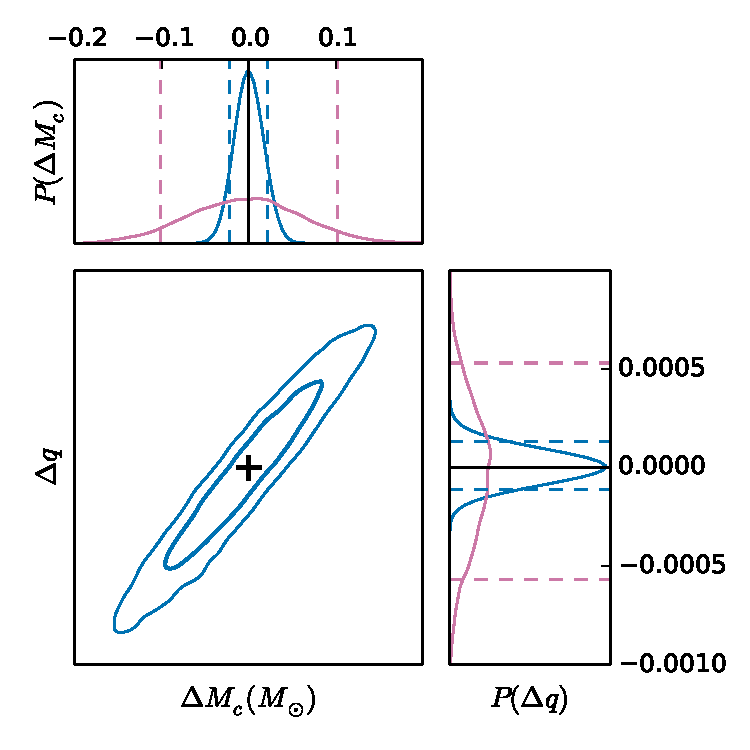
\includegraphics[width=3.4in]{figs/fig1_GR.pdf}
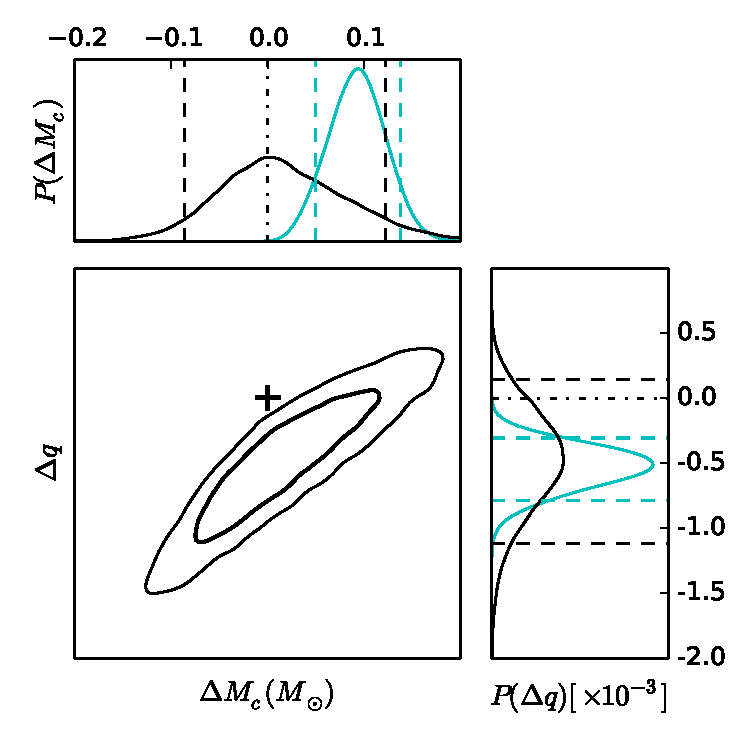
\includegraphics[width=3.4in]{figs/fig1_modGR.pdf}
\caption{\emph{Left:} The thick (thin) contours show the 68\% (95\%) credible regions in the joint posteriors of two parameters $\Delta M_c$ and $\Delta q$ that describe discrepancies in the estimated parameters using the quadrupole and non-quadrupole modes, estimated from a simulated GR signal. Black histograms on the side panels show the marginalized posteriors in $\Delta M_c$ and $\Delta q$, while the cyan histograms show the 1-dimensional posteriors in $\Delta M_c$ and $\Delta q$ estimated from the data by introducing only one variation (say, $\Delta M_c$) at a time, keeping the other fixed (say, $\Delta q = 0$). It can be seen that the posteriors are fully consistent with the GR prediction of $\Delta M_c = \Delta q = 0$ (shown by a ``+'' sign in the center panel and by thin black likes in side panels).  The simulated GR signal corresponds to a binary with total mass $M = \red{XX}M_\odot$ and mass ratio $q = 9$ and an inclination angle $\iota = \red{XX}$ obserbed by a single Advanced LIGO detector with an optimal SNR of 25. \emph{Right:} Same as the left plot except that the simulated signal contains a deviation from GR as described in the text. It can be seen that the posteriors are inconsisent with the GR expectation.}
\label{fig:contour_plots}
\end{center} \end{figure*}
%%%%%%%%%%%%%%%%%%%%%%%%%%%%%%%%%%%%%%%%%%%%%%%%%%%%%%%%%%%%%%%%%%%%%%%%%%%%%%%%%%%%%%%%%%

An interferometric GW detector observes a linear combination of the two polarizations $h_+(t)$ and $h_\times(t)$ of the GW signal, given by 
\begin{equation}
h(t) = F_+(\theta, \phi, \psi) \, h_+(t-t_0) + F_{\times}(\theta, \phi, \psi)\, {h}_{\times}(t-t_0), 
\label{eq:det_response}
\end{equation}
where $F_+$ and $F_x$ are the antenna pattern functions of the GW detector, $t_0$ is the time of arrival of the signal at the detector, and $(\theta, \phi, \psi)$ define the sky position and polarisation of the GW source respectively. The two GW polarizations $\h := h_+(t) - i \, h_\times(t)$ can be expanded in a basis of spin $-2$ weighted spherical harmonics, as:
\begin{equation}
\h(t; \iota, \phi_0, \blambda) = \sum _{\ell=2}^{\infty} \sum _{m=-\ell}^{\ell} \Ylm (\iota, \phi_0) \, \frac{{\h}_{lm}(t; \blambda)}{d_L}, 
\label{eq:spherical_harmonics}
\end{equation}
where $\Ylm$ are the basis functions of spin $-2$ spherical harmonics, $(\iota, \phi_0)$ define the direction of radiation in the source frame, $d_L$ is  the luminosity distance to the binary, and ${\h}_{lm}(t; \blambda)$ are the spherical harmonic modes of the waveform, which are completely described by the intrinsic parameters $\blambda$ of the system. We assume that the black holes are non-spinning and the binary to be qusi-circular. Hence $\blambda$ consists of only the masses $m_1$ and $m_2$ of the black holes. 

In GR, the set of intrinsic parameters $\blambda$ completely determines the multipolar structure of the waveform ${\h}_{lm}(t)$. Any inconsistency between the different multipoles of the radiation can point to a deviation from GR. In this paper, we propose a test of GR based on the consistency of different multipoles of the gravitational radiation from binary black holes. In order to formulate a consistency test between different multipoles, we rewrite Eq.(\ref{eq:spherical_harmonics}) by splitting the contributions from the dominant $(\ell = 2, m = \pm 2)$ mode of gravitational radiation, and the sub-dominant (higher order) modes 
\begin{eqnarray}
\h(t; \iota, \phi_0, \blambda, \Delta \blambda) & = & \sum_{m = \pm2} Y^{-2}_{2m} (\iota, \phi_0) {\h}_{2m}(t, \blambda)  \nonumber \\ 
 & + & \sum _{\text{H.O.M}} \Ylm (\iota, \phi_0) \h_{lm}(t, \blambda+\Delta \blambda)
\label{eq:test_HM}
\end{eqnarray}
where the subscript H.O.M underneath the summation in the second term on the RHS indicates contribution from just the higher-order multipoles of the gravitational radiation. Note that we allow a possibility of inconsistency between the dominant mode and higher order modes by introducing a deviation $\Delta \blambda$ in the set of intrinsic parameters that describe the higher order modes; in GR,  $\Delta \blambda = 0$. 

The data $d(t)$ contains the observed signal $h(t)$ given in Eq.~(\ref{eq:det_response}) along with noise, which is modeled as a stationary Gaussian random process 
\begin{equation}
d(t) = n(t) + h(t). 
\label{eq:detector_strain}
\end{equation}
For coalescencing binary black hole (BBH) systems in quasi-circular orbits, the observed signal $h(t)$ is described by a set of \emph{intrinsic} parameters $\blambda = \{m_1, m_2\}$ and \emph{extrinsic} parameters  $\btheta := \{t_0, \phi_0, d_L, \theta, \phi, \psi, \iota\}$ in GR. We also introduce a set of parameters $\Delta \blambda$ describing deviations from GR. The combined set of parameters is denoted as $\bxi = \{\blambda, \btheta, \Delta \blambda\}$.  Given data $d$ and assuming a particular model of the waveform as our hypothesis $H$, it is possible to compute the posterior distribution of the set of parameters ${\bxi}$ making use of the Bayes theorem, which states: 
\begin{equation}
P({\bxi} \, | \, d, H) = \frac{P({\bxi} \, | \, H) \, P (d \, | \, {\bxi}, H)}{P(d \, | \, H)}
\label{eq:Bayes_theorem}
\end{equation} 
The first term of the numerator on the RHS, $P({\bxi} \, | \, H)$ is the \emph{prior} distribution of the parameters ${\bxi}$, the second term $P (d \, | \, {\bxi}, H)$ is the \emph{likelihood} function, and the term in the denominator $P(d \, | \, H)$ is a normalisation constant, called the \emph{evidence}. For stationary Gaussian noise with power spectral density $S_n(f)$, the likelihiood can be written as:
\begin{equation}
P (d \, | \, {\bxi}, H) = \text{exp}\Big[ -\frac{1}{2}\int_{f_\mathrm{low}}^{f_\mathrm{high}} \frac{|\tilde{d}(f) - \tilde{h}(f;{\bxi}, H)|^2}{S_n(f)}df\Big]
\end{equation}
where $f_\mathrm{low}$ and $f_\mathrm{high}$ define the sensitivity bandwidth of the detector, while $\tilde{d}(f)$ and $\tilde{h}(f)$ are the Fourier transforms of $d(t)$ and $h(t)$, respectively. 

Using the above definition for the likelihood function, one proceeds to estimate $\bxi$ by stochastically sampling over the entire parameter space of interest. In this work, we use the \textsc{emcee}~\cite{goodman2010ensemble,foreman2013emcee} package, an ensemble Markhov chain Monte-Carlo (MCMC) sampler. \textsc{emcee} uses the underlying property of affine invariance of all Gaussian distributions to sample from highly skewed distributions faster than standard single-particle methods, such as Metropolis-Hastings implementations. A MCMC scheme is a random walk through the parameter space $\bxi$ generating samples of $\bxi$ with a probability density which ultimately converges to the stationary distribution of the Markhov chain, the posterior PDF $P(\bxi|d, H)$, using the equation of detailed balance. An \emph{ensemble} MCMC sampler implements a coordinated random walk of multiple ``walkers" through the parameter space, such that each step of the Markhov chain, or updating the position of any one walker at a paricular time step, is influenced by the positions of the rest of the walkers. The algorithm requires the hand-tuning of a small set of 1-2 parameters, and can be easily parallelised to use multiple CPU cores, giving it major advantages over traditional MCMC algorithms. From the posterior distribution $P(\bxi | d, H)$ of the full parameter set, we construct the posterior distribution $P(\Delta \blambda | d, H)$ of the set of parameters describing deviation from GR prediction, by marginalizing the posterior over all other parameters $\{\blambda, \btheta\}$. If the data is consistent with GR, we expect $P(\Delta \blambda | d, H)$ to be consistent with zero. 

\paragraph{Simulations using GR waveforms:---}
Here we demonstrate this test making use of simulated GW observations from binary black holes where the waveforms are modelled after the GR prediction. We employ the recent waveform model proposed by Mehta \etal~\cite{Mehta:2017jpq}, which provide accurate Fourier-domain models of the following spherical harmonic modes $\h_{\ell m}(f)$ of the expected GW from non-spinning binary black holes: $(\ell = 2, m = \pm2)$, $(\ell = 2, m=\pm1)$, $(\ell = 3, m=\pm3)$, $(\ell = 4, m = \pm4)$. GW observations are simulated by combining these signals with stationary Gaussian noise with power spectral density anticipated in Advanced LIGO's ``high-power, zero-detuning'' configuration~\cite{aLIGOZeroDetHighPower} making use of Eqs.~(\ref{eq:det_response}) and (\ref{eq:det_response}). We employ various choices for the binary's masses as well as orientations. 
 
We perform the test by introducing variations in the higher order modes: The higher-order modes $\hlm(f; \blambda+\Delta\blambda)$ are generated by introducing an extra parameter $\Delta\blambda$ while the quadrupole-modes $\h_{2\pm2}(f; \blambda)$ are generated by using the standard set of parameters $\blambda$ in GR. 

 We have experimented with different choices for the deviation parameter $\Delta\blambda$ --- both by introducing one deviation parameter at a time ($\Delta\blambda = \{\Delta M_c\}$ or $\Delta\blambda = \{\Delta q\}$ where $M_c$ is the chirp mass and $q := m_1/m_2$ is the mass ratio of the binary) and by introducing a combined deviation in two parameters $\Delta \blambda = \{\Delta M_c, \Delta q\}$. We show in Fig.~\ref{fig:contour_plots} (left plot) the results of the tests perforemd by varying either one parameter or two parameters, for the system with total mass $M := m_1 + m_2 = 80M_{\odot}$, mass ratio $q=9$, inclination angle $ {\iota}=60^{\circ} $ producing a signal-to-noise ratin  (SNR)  of 25 (SNR in higher modes is $\sim 10$). It can be seen that the results are consistent with the expected value in GR. As expected, the width of the posteriors are smaller when only one variation is introduced at a time. 

Figure~\ref{fig:dMc_dq_posteriors_gr} shows the expected width of the 90\% credible regions of the posteriors of the parameters describing deviations from GR, for the case of binaries with different masses, mass ratios and inclination angles. For all cases, the SNR of the injections is set to \red{XX}.  

\begin{figure}[h]
	\includegraphics*[width=3.5in]{figs/fig3.pdf}
	\caption{This figure shows the 90$\%$ width of $\Delta \blambda/\blambda$ where $\blambda$=M for various configurations of total mass $40M_{\odot}$.The best results of the test can be seen in the systems with high mass ratio.}
	\label{fig:dMc_dq_posteriors_gr}
\end{figure}


\paragraph{Simulations using modified-GR waveforms:---}

We also investigate the efficacy of our test in detecting deviations from GR. We introduce a deviation from GR in the simulated signals --- a propagation effect predicted by the Chern-Simons (CS) gravity. Under the CS modification to GR, a circularly polarised plane GW, propagating on an Friedmann–Lema\^itre–Robertson–Walker spacetime, would show amplitude birefringence and parity violation~\cite{Yunes:2010yf}. Compared to GR, right circularly polarised waves will be exponentially enhanced or suppressed with respect to left circularly polarized waves, as they propogate. That is, 
% 
\begin{equation}
\h_\mathrm{R,L}^\mathrm{mod} = \h_\mathrm{R,L} \, e^{-i \, \delta\phi_\mathrm{R,L}} \simeq  \h_\mathrm{R,L} \, (1 -i \, \delta\phi_\mathrm{R,L}),
\label{eq:cs_modification_h}
\end{equation}
where $\h_\mathrm{R,L} = (h_+ \pm h_\times)/\sqrt{2}$ are the right/left circularly polarized polarization states predicted by GR and $\delta \phi_{R,L}$ is an additional phase contribution due to the CS correction, given by 
\begin{equation}
\delta \phi_\mathrm{R,L}= \pm i \, f \, \pi \, z \, \Big(\dot{\theta_0}-\frac{\ddot{\theta_0}}{H_0}\Big).
\label{eq:cs_modification_dphi}
\end{equation}
Here, $f$ is the Fourier frequency measured by the observer, $z$ is the cosmological redshift at source, and ${H_0}$ is the value of the Hubble constant measured by the observer, while $\dot{\theta_0}$ and $\ddot{\theta_0}$ denote the first and second time-derivative of the CS coupling field. Note that the CS correction is purely imaginary which results in amplitude birefringence. Solar system observations of the LAGEOS satellites have allowed us to derive a bound $|\dot{\theta_0}-\frac{\ddot{\theta_0}}{H_0}| < 2000~\mathrm{km}$~\cite{Yunes:2010yf,Smith:2007jm}.

From the $+,\times$ polarizations of the GR waveforms discussed in the earlier section, we construct a modified-GR waveforms by introducing the propagation effects described in Eq.\eqref{eq:cs_modification_h}, with $\dot{\theta_0}-\frac{\ddot{\theta_0}}{H_0} = 2000~\mathrm{km}$. Example of such a modified waveform is shown in Fig.~\ref{fig:mod_gr_waveform} for a system $M = 80M_{\odot}$, $q =9$, $\iota = 90^{\circ}$,solar system constraint at a distance of 200Mpc. We inject this waveform into simulated noise and perform the Bayesian parameter estimation described earlier. The resulting injected waveform has an optimal SNR of \red{XXX} in the detector, of which \red{$\sim XX\%$} is distributed in the non-quadrupole modes. Figure~\ref{fig:contour_plots} (right panel) shows the posteriors on parameters describing describing deviations from the GR prediction. It can be seen that the posteriors on deviation parameters $\{\Delta M_c, \Delta q\}$ are inconsistent with the GR prediction, $\{0, 0\}$. 

\begin{figure}[h]
	\includegraphics*[width=3.1in]{figs/mod_GR_waveform.pdf}
	\caption{Amplitudes of GR and modified GR waveform with the modification $\delta \phi_\mathrm{R,L} = \pm i \, 10^{-3} f$ [see, Eq.\eqref{eq:cs_modification_dphi}]. The system configuration is $M = 80 M_{\odot}$, $q = 9$, $\iota=90^{\circ}$ at a distsance of 200 Mpc. The match between GR and mod.GR waveform is greater than 0.96 for such a departure.}
\label{fig:mod_gr_waveform}
\end{figure}

\paragraph{Conclusions and future work:---} In this paper, we proposed a new method to test the consistency of an observed GW signal with a binary black hole system predicted by GR. The test relies on the fact that, given the parameters of a binary system, the multipolar structructure of the radiated GW signal is uniquely predicted by GR. Thus, if we estimate the parameters of the binary from different spherical harmonic modes of the observed signal independently, those estimates have to be consistent with each other. Any incosistency between the different estimates will point to a deviation from GR. We developed a Bayesian parameter estimation method to identify potential deviations from GR predictions and tested this method using simulated signals in GR, as well as simulated signals containing certain deviations from GR.  We provided the first estimates of the expected precision of such tests that can be performed using GW observations of binary black holes anticipated by LIGO and Virgo in the next few years. 

Note that, this test requires the observation of GW signals where the non-quadrupole modes can be observed with appreciable SNR. This will require binaries with large mass ratios ($q \gtrsim 3$) and inclined orientations ($\iota \gtrsim 45^{\circ}$). Thus, this test can not be performed on the GW signals observed by LIGO and Virgo during their first two observational runs, for which mass ratios are close to 1 and inclinations are closed to face-on ($\iota \simeq 0$). The detection rates of binaries with large mass ratios depend on the astrophysical merger rates of such binaries, which is currently uncertain, while the detection rate of binaries with large inclination angle is related to the same with small inclination angles by a simple geometric factor. 

Note that in this paper we assume, for simplicity, that the black holes in the binary have negligible spins. The method can be easily generalized to the case of binaries consisting of spinning black holes. Indeed, the systematic errors due to inaccuracies in the waveform modeling and detector calibration errors need to be understood before implementing such a test on real observations. We leave these as future work. 

\paragraph{Acknowledgments:---}
This research was supported by the Indo-US Centre for the Exploration of Extreme Gravity funded by the Indo-US Science and Technology Forum (IUSSTF/JC-029/2016). P.~A.'s research was, in addition, supported by a Ramanujan Fellowship from the Science and Engineering Research Board, India and by the Max Planck Society through a Max Planck Partner Group at ICTS-TIFR. Computations were performed at the ICTS cluster Alice. 
%
\bibliographystyle{apsrev-nourl}
\bibliography{TGR_HM}

\end{document}
